\documentclass[tikz,border=3pt]{standalone}
\usepackage{amsmath}
\usepackage{tikz}
\usetikzlibrary{calc,positioning,arrows.meta}

% 统一样式
\tikzset{
  bar/.style={draw, line width=0.6pt, minimum width=1.6mm, minimum height=30mm},
  label/.style={font=\small},
}

% 成对竖条命令:\pair{name}{(x,y)}{height}{sep}
\newcommand{\pair}[4]{%
  \coordinate (#1c) at #2;
  \node[bar, minimum height=#3, anchor=center] (#1l) at ($(#1c)+(-#4/2,0)$) {};
  \node[bar, minimum height=#3, anchor=center] (#1r) at ($(#1c)+(#4/2,0)$) {};
}

\begin{document}
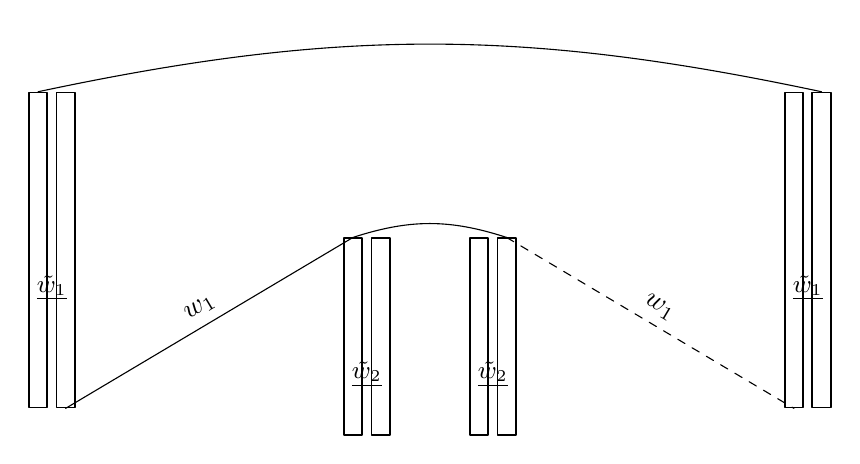
\begin{tikzpicture}[x=1cm,y=1cm, line cap=round, line join=round]
  % 内间距(同组两条之间)
  \def\sep{3.5mm}

  % 四组竖条:左右高、中间低(坐标可按需要微调)
  \pair{A}{(0,0)}     {4.0cm}{\sep} % 左高组
  \pair{B}{(4.0,-1.1)}{2.5cm}{\sep} % 中左低组
  \pair{C}{(5.6,-1.1)}{2.5cm}{\sep} % 中右低组
  \pair{D}{(9.6,0)}   {4.0cm}{\sep} % 右高组

  % 组下方标签(带下划线)
  \node[label, below=2mm of Ac] {$\underline{\tilde{w}_1}$};
  \node[label, below=2mm of Bc] {$\underline{\tilde{w}_2}$};
  \node[label, below=2mm of Cc] {$\underline{\tilde{w}_2}$};
  \node[label, below=2mm of Dc] {$\underline{\tilde{w}_1}$};

  % 顶部大弧线(左高组→右高组)
  \draw (Al.north) to[bend left=12] (Dr.north);

  % 中部小弧线(中左→中右)
  \draw (Bl.north) to[bend left=18] (Cr.north);

  % 左侧斜连线,标 w1
  \draw (Ar.south) -- node[midway, above, sloped] {$w_1$} (Bl.north);

  % 右侧斜连线(虚线),标 w1
  \draw[dashed] (Cr.north) -- node[midway, above, sloped] {$w_1$} (Dl.south);
\end{tikzpicture}
\end{document}